%%% File encoding: UTF-8
%%% äöüÄÖÜß  <-- keine deutschen Umlaute hier? UTF-faehigen Editor verwenden!

%%% Magic Comments zum Setzen der korrekten Parameter in kompatiblen IDEs
% !TeX encoding = utf8
% !TeX program = pdflatex 
% !TeX spellcheck = de_DE
% !BIB program = biber

\documentclass[bachelor,german]{hgbthesis}
% Zulässige Optionen in [..]: 
%   Typ der Arbeit: diploma, master (default), bachelor, internship 
%   Hauptsprache: german (default), english
%%%----------------------------------------------------------

\RequirePackage[utf8]{inputenc}		% bei der Verw. von lualatex oder xelatex entfernen!

\graphicspath{{images/}}    % Verzeichnis mit Bildern und Grafiken
\logofile{logo}				% Logo-Datei = images/logo.pdf (\logofile{}, wenn kein Logo gewünscht)
\bibliography{references}  	% Biblatex-Literaturdatei (references.bib)

%%%----------------------------------------------------------
% Angaben für die Titelei (Titelseite, Erklärung etc.)
%%%----------------------------------------------------------

%%% Einträge für ALLE Arbeiten: -----------------------------
\title{Interaktion Hands-Free. Eine Analyse alternativer Interaktionsmöglichkeiten}
\author{Hanna\ Wagner}
\programname{Kommunikation, Wissen, Medien}
\placeofstudy{Hagenberg}
\advisor{FH-Prof. DI (FH) Dr. Mirjam Augstein}
%\dateofsubmission{2017}{02}{28}	% {YYYY}{MM}{DD}

%%% Zusätzlich für eine Bachelorarbeit: ---------------------
\thesisnumber{S1410456033}   % Stud-ID, z.B. 1310238045-A  
% (A = 1. Bachelorarbeit)
\semester{Sommersemester 2017} 
%\coursetitle{ } 


%%%----------------------------------------------------------
\begin{document}
%%%----------------------------------------------------------

%%%----------------------------------------------------------
\frontmatter                    % Titelei (röm. Seitenzahlen)
%%%----------------------------------------------------------

\maketitle
\tableofcontents
\listoffigures

%\include{thesis_DE/front/vorwort} % Optional. Ggf. weglassen
\chapter{Kurzfassung}

%kurze einleitung
Die folgende Arbeit gibt einen Einblick in verschiedene alternative Ein- und Ausgabemethoden, vergleicht die einzelnen Systeme miteinander und beschreibt deren Einsatzgebiete.
\newline \newline
%die fünf eingabemethoden, ev kurz beschreiben wie sie funktioniren
Alternativ zur Interaktion mit einem Systems mit Hilfe der Hände, gibt es die Möglichkeit durch Sprachsteuerung, Augensteuerung, Gestensteuerung, Muskelsteuerung oder durch Steuerung basierend auf Gehirnaktivität mit einem Computer zu interagieren. Bei der Sprachsteuerung wird das Gesprochene digital erfasst, mit bereits bestehenden Mustern und Wortlauten verglichen, um so den Inhalt zu erfassen und die gewünschte Aktion durchzuführen. Bei der Augensteuerung wird sowohl mit Kameras die Augenbewegungen am Bildschirm mitverfolgt, als auch gleichzeitig von einer Software in beispielsweise Mausbewegungen parallel umgewandelt. Die Gestensteuerung kann in mehrere einzelnen Gesten aufgeteilt werden. Zusammenfassend kann jedoch gesagt werden, dass meist ein joystickähnliches Element für die Bewegungsrichtung verwendet und zusätzliche Tasten bei der Auswahl von gewünschten Symbolen oder Elementen helfen. Die Erfassung von elektromyografischen Daten (EMG) bieten die Grundlage für die Muskelsteuerung. Der Benutzer kann durch gezieltes An- und Entspannen der Muskel die gewünschte Interaktion herbeiführen. Die Steuerung durch Gehirnaktivität funktioniert über die Messung der Wellen im menschlichen Gehirns mit Hilfe eines  Elektroenzephalografen (EEG). Erhöhte Gehirnaktivität in den einzelnen Bereichen kann in Befehle bzw. in eine Interaktion umgewandelt werden.
\newline \newline
%ausgabe
Ein Computer hat die Möglichkeit durch auditive, haptische oder visuelle Ausgabe dem Benutzer Feedback geben zu können. Diese Ausgabemethoden sind allerdings nicht zwingend an bestimmte Eingabemethoden gebunden. So gibt es nicht nur bei Systemen, die über die Sprache gesteuert werden, ein akustisches Feedback, sondern beispielsweise auch bei Muskelsteuerungssystemen.
\newline \newline
%vergeleich, einsatzgebiete
Als Konklusion finden alternative Interaktionsmöglichkeiten Einsatz in alltäglichen Situationen, im Arbeitsleben und als assistive Technologien. Auf Grund des momentanen Beliebtheitsgrades von Amazon Alexa und weiteren Sprachassistenten wurde die Sprachausgabe als die beliebte Art alternativen Interaktionssystem im Moment definiert. Hingegen werden bei der Steuerung durch Gehirnaktivität die meisten Potentiale gesehen.
		
\chapter{Abstract}

\begin{english} %switch to English language rules
The following paper provides an insight into various alternative input and output methodes, compares all the individual systems with each other and describes their application areas.
\newline \newline
There are various posibiliets how a user can interact with a system without using the hands. There is the option to interact using voice control, eye control, gesture control, muscle control or control based on brain activity. In case of speech control the spoken words are first saved digitally. Later they are compared with existing patterns and word orders to understand the content and required action of the user. When a user interacts with an eye control system the eye movement will be tracked by one or more cameras and a software translates theis movements into real time mouse movements. As a third method the gesture control will be described, which can divied in serveral sub-categories. All in all they all use a joystick-like element for the direction of movement and additional keys help with the selection of desired symbols or elements. Electromyographic data (EMG) are providing the basis for muscle control. The user can achieve the desired interaction through targeted muscle contraction and relaxation. The control by brain activity utilizes the measurement of the human brain waves with the help of an electroencephalograph (EEG). Increased brain activity in the specific areas can be converted into control commands or into an interaction in general.
\newline \newline
In addition various ouput methods are explained. A computer can give feedback either through audio, hapitc or visual output.
\newline \newline
Alternative interaction options are used in everyday situations, at work and as assistive technologies. Due to the current popularity of Amazon Alexa and other language assistants, the language output was defined as the most popular type of alternative interaction systems at the moment. On the other hand shows the control of brain activity the most potential.
%hier Abstract hinschreiben
\end{english}


			

%%%----------------------------------------------------------
\mainmatter          % Hauptteil (ab hier arab. Seitenzahlen)
%%%----------------------------------------------------------

\chapter{Einleitung}
\label{cha:Einleitung}

\section{Motivation und Zielsetzung}
%
Die meisten Interaktionen mit elektronischen Geräten jeder Art finden durch den Einsatz unserer Hände statt. Das reicht von der einfachen Bedienung von Geräten (z.B. Einschalten eines Computers) bis hin zur Steuerung von Abläufen mittels Gestik (z.B. Liederwechsel durch eine Wischgestik, die von einer Software erkannt und in einen Befehl umgewandelt wird). Doch nicht immer gibt es die Möglichkeit mit Hilfe der Hände zu interagieren. Beispielsweise sollen beim Autofahren beide Hände am Lenkrad bleiben, bei anstrengenden und präzisen Arbeiten an Maschinen müssen oft beide Hände benutzt werden oder aber auch für Menschen mit Tetraplegie bzw. Tetraparese, die ihre Hände und Arme nicht oder oft nur sehr eingeschränkt benutzen können, sind alternative Interaktionsmöglichkeiten äußerst nützlich.
\newline \newline
Ziel der Arbeit ist es einen umfassenden Überblick mit samt der Vor- und Nachteile, sowie Einsatzgebiete über alternative Eingabe- und Ausgabemethoden zu geben.

\section{Aufbau}
%Kapitel 2
Kapitel ~\ref{cha:Eingabe} stellt die einzelnen Eingabemethoden vor. Diese werden einerseits aus einer technischen Sicht (wie funktioniert das System), andererseits aus der Interaktionssicht (was muss ein Benutzer für eine erfolgreiche Interaktion machen bzw. beachten) beschrieben.
\newline \newline
%Kapitel 3
Anschließend werden in Kapitel ~\ref{cha:Ausgabe} Ausgabemethoden vorgestellt. Diese Ausgabemethoden müssen nicht unbedingt an eine bestimmte Eingabemethode gebunden sein. Das bedeutet, dass beispielsweise Systeme, die mit Hilfe der Augen gesteuert werden, auch ein akustisch Feedback geben können. 
%Kapitel 4
\newline \newline
Abschließend werden in Kapitel ~\ref{cha:Vergleich} die Vor- und Nachteile der einzelnen alternativen Eingabemöglichkeiten erläutert, gesonderte Rahmenbedingungen vorgestellt und Einsatzgebiete zu den einzelnen Systemen beschrieben.








\chapter{Eingabemethoden}
\label{cha:Eingabe}

Es gibt viele Anwendungsfälle, in denen die Interaktionen mit einem System mit den Händen nicht möglich ist. In alltäglichen Situation, wie beispielsweise beim Autofahren, bei anstrengenden und präzisen Arbeiten an Maschinen oder für Menschen mit Beeinträchtigung, sind Alternativen notwendig. Aus diesem Grund beschäftigt sich dieses Kapitel mit verschiedenen alternativen Eingabemethoden, die es auch ohne den Einsatz von den Händen ermöglichen, mit einem System interagieren zu können. Vor- und Nachteile, gesonderte Rahmenbedingungen und Einsatzgebiete werden in Kapitel~\ref{cha:Vergleich} näher erläutert. 

%%%%%%%%%%%%%%%%%%%%%%% SPRACHSTEUERUNG %%%%%%%%%%%%%%%%%%%%%%%%%%%
\section{Sprachsteuerung}

Eine Alternative zur Interaktion mit den Händen stellt die Steuerung mit Hilfe der menschlichen Stimme dar. Ein Spracherkennungssystem soll im optimalen Fall das Gesprochene genau so gut erkennen und verstehen können wie ein Mensch. Da es unterschiedliche Sprachangewohnheiten, einen unterschiedlichen Dialekt und es auch syntaktische Unterschiede gibt, kann ein System an das menschliche Verstehen allerdings nur angenähert werden. Oft werden daher in der Praxis die Systeme speziell für einzelne Szenarien entwickelt bzw. angepasst. 
\newlinew \newline
Wird der Inhalt des Gesprochen analysiert, wird dies als Spracherkennung bezeichnet. Hier gibt es zwei Ansätze, damit das System das Gesprochene versteht:
\begin{itemize}
      \item Mustervergleich
      \item Statistische Spracherkennung
\end{itemize}
\vspace{\baselineskip}
Bei einem Mustervergleich werden die gesprochenen Wörter mit den bereits abgespeicherten Mustern und Begriffen verglichen. Jenes Wort, das dem Eingabewort am ähnlichsten ist, wird verwendet. Hingegen werden bei der statistischen Spracherkennung Beschreibungen von Lauten und Wörtern verwendet. Zusätzlich wird berechnet, welche Wortfolgen am wahrscheinlichsten sind. Hierbei werden einzelne Sequenzen des Gesprochenen verwendet und analysiert. Die Wahrscheinlichkeiten für die Wortfolgen können entweder auf einer bestehenden Statistik basieren, oder das System lernt von Eingabe zu Eingabe mit und muss für eine sichere Vorhersage im Vorhinein trainiert werden \cite{KaufmannPfisterSprache}. 
\newline \newline
%technischer aspekt
Bevor das Signal im gesamten Prozess bei dem Analyseschritt angelangt, durchläuft die Analysesequenz zuvor noch einige Prozessschritte. Wenn eine Person etwas spricht werden die analogen Wellen durch elektroakustische Wandler (zum Beispiel ein Mikrophon) in ein elektrisches Signal (Sprachsignal) umgewandelt, damit der Computer diese interpretieren und weiterverarbeiten kann. Anschließend werden auf den gespeicherten Daten verschiedenste Filter angewendet, um störende Signale, wie zum Beispiel Hintergrundgeräusche oder Pausen während des Sprechens zu entfernen. Erst dann kann im nächsten Schritt das System das Gesprochene mit Hilfe eines Mustervergleichs oder einer statistischen Spracherkennung analysieren und so den Sinn erfassen. Ist der Inhalt des Gesprochenen bekannt, kann dieser in einen Text und somit in einen Befehl umgewandelt und dadurch der Computer bzw. das Programm gesteuert werden \cite{KaufmannPfisterSprache}.
\newline \newline
Es gibt viele Faktoren, die einen Einfluss auf das Sprachsignal haben. So hat jeder Mensch neben seiner einzigartigen Stimme einen unterschiedlichen Dialekt, Sprachgewohnheiten, Emotionen in der Sprache, Pausenangewohnheiten und eine verschiedene Sprechgeschwindigkeit \cite{KaufmannPfisterSprache}. Diese Komponenten sind nicht nur wichtig für die Erkennung, was gesprochen wird, sondern viel mehr dafür, wer spricht (Sprechererkennung).
\newline \newline
%Sprechererkennung
Um festzustellen zu können welche Person gerade spricht, muss es Referenzdaten im System geben, die mit dem aktuellen Signal verglichen werden können. Dies geschieht entweder, wenn die Person ein bestimmtes Signalwort spricht, das mit dem abgespeicherten Wort verglichen wird, oder wenn das Sprachsignal lange genug ist, kann auf Grund von statistischen Merkmalen wie z.B. Stimmfarbe oder Sprechgeschwindigkeit eine Übereinstimmung gefunden werden \cite{KaufmannPfisterSprache}. 
\newline \newline
%Interaktion!
Kommunikation durch Sprache ist eines der leichtesten, wenn nicht sogar das intuitivste Mittel zur Verständigung. Daher sollte auch die Interaktion mit einem Computer diesem hohen Standard entsprechen. Allerdings ist im Gegensatz zur gewohnten Face-to-Face-Kommunikation das Gegenüber im Bezug auf Spracherkennung kein intelligenter Gesprächspartner. Ein Computer kann nur schwer lange und komplizierte Sätze und Gedankengänge mitverfolgen und daraus schlecht eine Kernaussage ziehen. Daher muss dem System verständlich gemacht werden, wann es zuhören soll \cite{SpeechInteraction}.
Zwei gängige Methoden für den Start zur Interaktion sind:
\begin{itemize}
      \item das Drücken einer Starttaste
      \item das Aussprechen eines Aktivierungswortes
\end{itemize}
\vspace{\baselineskip}
Weil das Drücken eines Startknopfes die Hilfe der Hände benötigt, steht im Kontext dieser Arbeit das Aussprechen eines Aktivierungswortes zum Start der Interaktion im Vordergrund.
Durch das Wort 'Alexa' wird beispielsweise Amazon Echo%
Durch das Wort 'Alexa' wird beispielsweise Amazon Echo%
\footnote{https://www.amazon.com/Amazon-Echo-Bluetooth-Speaker-with-WiFi-Alexa/dp/B00X4WHP5E}
%
aktiviert. Bei Amazon Echo handelt es sich um ein Sprachinteraktionssystem, das beispielsweise Musik abspielen, den Einkauf bestellen oder auch Nachrichten und Wetterbeiträge zur Verfügung stellen kann.
Im Gegensatz zur Benutzung von Amazon Echo, muss bei der Sprachsteuerung von Apple (Siri)%
\footnote{https://www.apple.com/ios/siri/}
%
 das System erst auf die eigene Stimme eingestellt, also kalibriert werden. Das Aktivierungswort 'Hey Siri' muss drei Mal einzeln und zwei Mal in einem Satz eingesprochen werden, damit diese Funktion beispielsweise am iPhone freigeschaltet wird. Anschließend können ebenfalls Wetter oder Nachrichtendaten abgefragt werden, aber auch Anrufe oder Nachrichten können mit Hilfe der Stimme getätigt werden. 
\newline \newline
Sobald das System bereit ist die Eingabe aufzunehmen, muss beachtet werden, dass laut und deutlich gesprochen wird, keine zu große Distanz zum Mikrophon besteht und dass nicht zu schnell gesprochen wird.
\newline \newline
Zusammenfassend lässt sich sagen, dass die Sprachinteraktion mit dem Computer aus Benutzersicht noch einige Verbesserung braucht, damit die Bedienung natürlicher und intuitiver wird und der einer Face-to-Face-Kommunikation näher kommt.

%%%%%%%%%%%%%%%%%%%%%%% AUGENSTEUERUNG %%%%%%%%%%%%%%%%%%%%%%%%%%%
\section{Augensteuerung}
\label{cha:Augensteuerung}

Eine weitere alternative Interaktionsmöglichkeit stellt die Steuerung mit Hilfe der Augen dar. Eye-Tracking-Systeme werden verwendet, um die Augenbewegungen zu identifizieren. Parallel dazu wandelt eine Software die Augenbewegungen in einen Mauszeiger um, um so mit dem System interagieren zu können. 
\newline \newline
Um die Augenbewegungen nachvollziehen zu können, werden sowohl ein Infrarotlichtstrahl, als auch eine Videokamera auf das Auge fokussiert. Eine Software analysiert die Bewegungen im Hintergrund und erkennt, wo der Fokus auf dem Bildschirm liegt. Für die Umrechnung ist außerdem wichtig, dass die Position des Kopfes vom Interaktionssystem erkannt wird \cite{NielsenPernice}.
\newline \newline
Die Teilbereiche des Auges bzw. des menschlichen Sehens, die für die Augensteuerung relevant sind, sind das periphere und foveale Sehen. Das foveale Sehen beinhaltet jenen Teil, den das menschliche Auge als scharfen Bildausschnitt wahrnimmt, also auf welchen Ausschnitt es fokussiert. Hingegen enthält das periphere Sehen den Großteil unser Sehwahrnehmung. Dies beinhaltet jene Bereiche, die nicht fokussiert sind \cite{NielsenPernice}. Daher ist das foveale Sehen für die Augensteuerung relevant.
\newline \newline
Nielsen und Pernice \cite{NielsenPernice} unterscheiden beim menschlichen Sehen zusätzlich zwischen Fixation und Sakkaden. Das menschliche Auge bewegt sich nicht kontinuierlich, sondern ein Blick setzt sich aus schnellen Bewegungen mit Pausen dazwischen zusammen. Dies geschieht so schnell, dass es im Alltag nicht bewusst wahrgenommen wird. Wenn das Auge auf einem bestimmten Punkt ruht spricht man von Fixation. Die schnellen Zwischenbewegungen von einer Fixation zur nächsten werden Sakkaden genannt. Die Schwierigkeiten der Eye-Tracking-Systeme und der Augensteuerungssoftware bestehen darin, diese Fixationen zu erkennen, da diese meist zwischen einer hundertstel und einer zehntel Sekunde liegen \cite{NielsenPernice}.
%abbildung 2
\begin{figure}
\centering
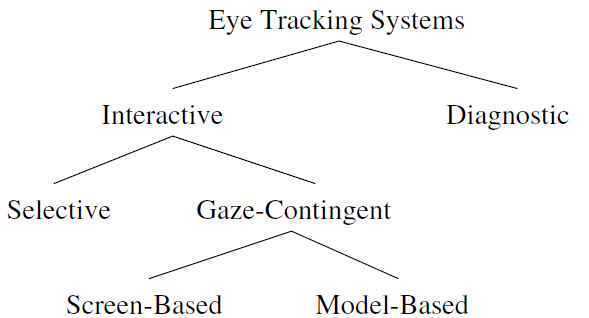
\includegraphics[width=.7\textwidth]{eyeTrackingSystems}
\caption{Hierachie von Eye-Tracking-Systemen \cite{Duchowski}.}
\label{fig:eyeTrackingSystems}
\end{figure}
\newline \newline
Wie in Abb.~\ref{fig:eyeTrackingSystems} dargestellt, unterscheidet Duchowski \cite{Duchowski} zwischen interaktiven und diagnostischen Systemen. Da bei diagnostischen Systemen keine direkte Interaktion stattfindet, sondern die Augenbewegungen aufgezeichnet und im Nachhinein ausgewertet werden, sind für die Analyse von Interaktionsmöglichkeiten ausschließlich interaktive Systeme relevant. 
\newline \newline
Interaktive Systeme lassen sich wiederum in zwei Bereiche teilen. Selektive Systeme benutzen den Blickpunkt als analoges Eingabeelement, während Blickkontingentsysteme für die Darstellung von komplexen Displays verwendet werden. 
\newline \newline
Abgesehen davon, wie die Daten aufgezeichnet werden bzw. was aufgezeichnet wird, gibt es eine Unterscheidung zwischen den verschiedenen Eye-Tracking-Systemen. Diese können in intrusive und nicht-intrusive Systeme unterteilt werden. Intrusive Eye-Tracker haben einen direkten Kontakt mit den Anwendern (z.B. durch Kontaktlinsen). Nicht-intrusive Eye-Tracking-Systeme hingegen messen die Blicke mit Hilfe einer oder mehrerer Kameras. 
\newline \newline
In der Praxis werden eine Vielzahl verschiedenster Eye-Tracking-Systeme als Basis für die Augensteuerung verwendet. Die Unternehmen Tobii%
\footnote{http://www.tobii.com/group/}
%
und SensoMotoricInstruments (SMI)%
\footnote{https://www.smivision.com/}
%
sind Spitzenreiter auf dem Gebiet des Eye-Tracking und verfügen über eine umfangreiche Produktpalette bzw. vielfältige Anwendungsgebiete. 
\begin{figure}
\centering\small
\setlength{\tabcolsep}{0mm}	% alle Spaltenränder auf 0mm
\begin{tabular}{c@{\hspace{-15mm}}c} % mittlerer Abstand = 12mm
  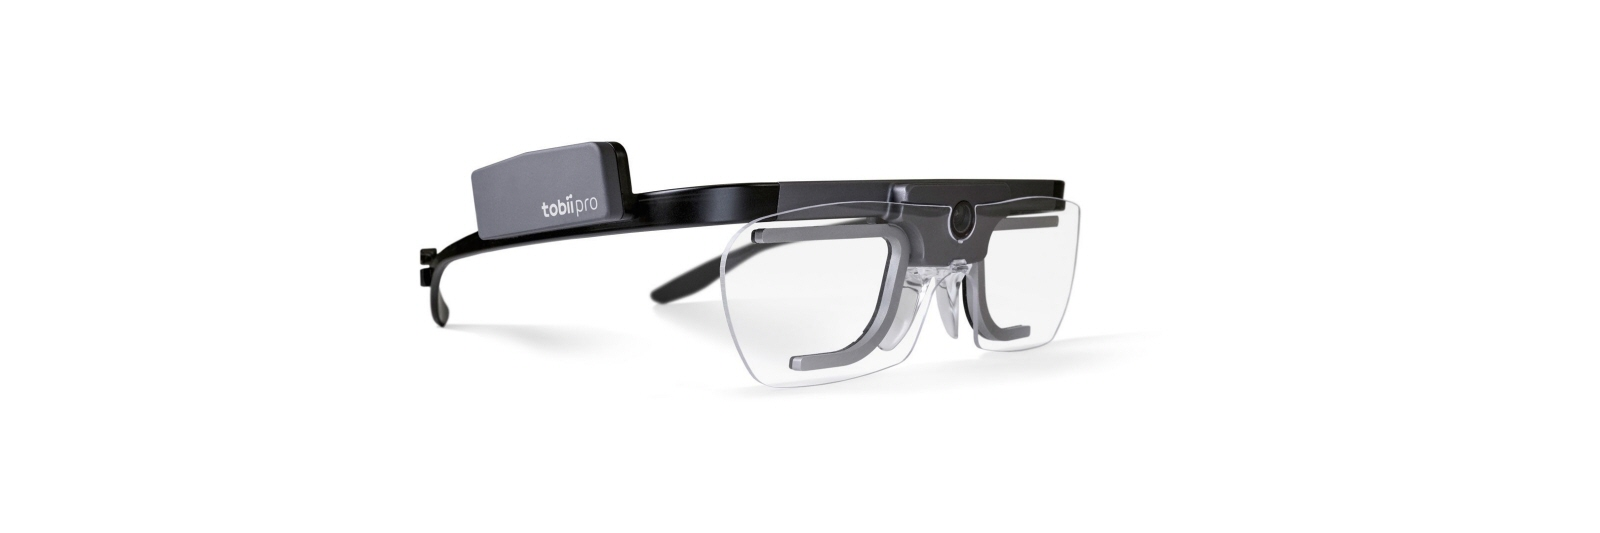
\includegraphics[width=.6\textwidth]{TobiiPro_Glasses} &
  
\includegraphics[width=.6\textwidth]{Tobii_Spectrum}
\\
  (a) & (b)
\\[4pt]	%vertical extra spacing (4 points)
  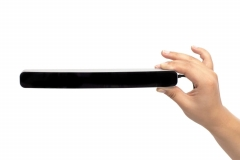
\includegraphics[width=.36\textwidth]{SMIRED}
\\
  (c)
\end{tabular}
%
\caption{Übersicht über die Eye-Tracking-Systeme von Tobii und SMI \newline
(a)~Tobii Pro Glasses 2 \cite{TobiiGlasses}, (b)~Tobii Pro Spectrum \cite{TobiiSpectrum} und (c)~SMI Red250mobile \cite{SMIRED}.}
\label{fig:Tobii}
\end{figure}
\newline \newline
In Abb.~\ref{fig:Tobii}(a) ist die tragbare Eye-Tracking-Brille Tobii Pro Glasses 2 zu sehen. Diese ist so gestaltet worden, um ein möglichst natürliches Nutzungsverhalten zu erzielen. Es müssen keine Voreinstellungen vorgenommen werden, die Brille kann sofort benutzt werden. Bei Tobii Pro Spectrum (Abb.~\ref{fig:Tobii}(b)) handelt es sich um ein nicht-intrusives System, das die Blickdaten mit einer Geschwindigkeit von bis zu 600 Hz aufnimmt. Das Unternehmen SMI hat, wie in Abb.~\ref{fig:Tobii}(c) zu sehen ist, ein mobiles Eye-Tracking-System entwickelt, das die Bewegungen mit bis zu 250 Hz aufzeichnen kann. Alle diese Systeme verwenden das Prinzip von Fixation und Sakkaden des Auges, um die Augenbewegungen nachvollziehen zu können. Damit nicht nur die Augenbewegungen aufgezeichnet werden, sondern eine Interaktion stattfinden kann, müssen diese Systeme in Kombination mit einer Software eingesetzt werden, die die Blicke in Mausbewegungen o.ä. umwandelt.
\newline \newline
Bevor ein Benutzer mit Hilfe der Augen beispielsweise eine Bildschirmtastatur bedien kann, muss das System bzw. die Software erst auf den Anwender eingestellt werden. Bei der Kalibrierung tauchen am Bildschirm nacheinander Symbole auf, die fixiert werden müssen. Dadurch können der Blickwinkel und der Augenabstand vermessen werden um eine optimale Interaktion zu erreichen. Bei der eigentlichen Anwendung erkennt das System dann, wenn der Blick auf einem Punkt länger verharrt, also scharf stellt. Verharrt der Blick also länger auf einem Buchstaben der Tastatur, wird dies als Mausklick gewertet und der Buchstabe oder das Symbol ausgewählt. Am Beispiel von Seetech von Humanelektronik%
\footnote{http://humanelektronik.de/}
%
beträgt die Fixationszeit etwa 0.5 bis 1.5 Sekunden \cite{SEETECH}.
\newline \newline \newline
Zusammenfassend kann gesagt werden, dass für die Interaktion mit einer Anwendung bzw. einem System interaktive Eye-Tracking-Systeme für die Nachvollziehbarkeit der Augenbewegungen und zusätzlich eine Software für die Umrechnung in Mausbewegungen relevant sind. Nach einer kurzen Kalibrierung können durch Fixation einzelne Elemente auf dem Bildschirm ausgewählt und auf Grund der Fixationszeit in einen Mausklick umgewandelt werden.

%%%%%%%%%%%%%%%%%%%%%%% Gestensteuerung %%%%%%%%%%%%%%%%%%%%%%%%%%%
\section{Gestensteuerung}

Eine weitere Alternative zur Interaktion mit den Händen stellt die Gestensteuerung dar. Mit Hilfe von Gesten kann eine Handlung mit verschiedenen Teilen des Körpers (\zB den Händen, Füßen, Kopf) zum Ausdruck gebracht werden. In diesem Abschnitt bezieht sich die Gestensteuerung auf alle Körperteile ausschließlich der Hände. In der Literatur werden Gesten unterschiedlich definiert, in diesem Zusammenhang versteht man unter einer Geste \cite{PreimDachselt}:
\begin{quote} ...die Bewegung von Fingern, Händen und Armen - oder auch weiterer Körperteile, wie Kopf, Augen und Lippen - aufgrund einer kommunikativen Absicht. Damit enthält die Bewegung als solche signifikante Informationen, die an den Computer übermittelt werden sollen. \end{quote}
In diesem Abschnitt werden Kinn-, Mund-, Kopf- sowie Fußsteuerung näher erläutert. 
%
%
%%%%%%%%% Kinnsteuerung %%%%%%%%%
\subsection{Kinnsteuerung}
\label{cha:Kinnsteuerung}

Bei der Kinnsteuerung werden mit Hilfe des Kinns Bewegungen ausgeführt, um mit einem System interagieren zu können. Die unterschiedlichen Möglichkeiten werden anhand der nachfolgenden Beispiele erklärt.
%
\begin{figure}
\centering\small
\setlength{\tabcolsep}{0mm}	% alle Spaltenränder auf 0mm
\begin{tabular}{c@{\hspace{15mm}}c} % mittlerer Abstand = 12mm
  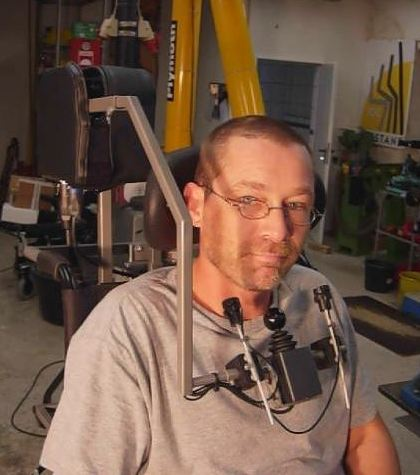
\includegraphics[width=.3\textwidth]{moso_kinn} &
  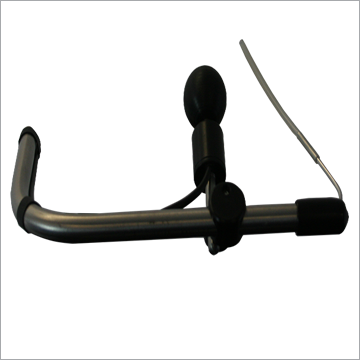
\includegraphics[width=.3\textwidth]{smilesmart_kinn}
\\
  (a) & (b)
\\[5pt]	%vertical extra spacing (4 points)
  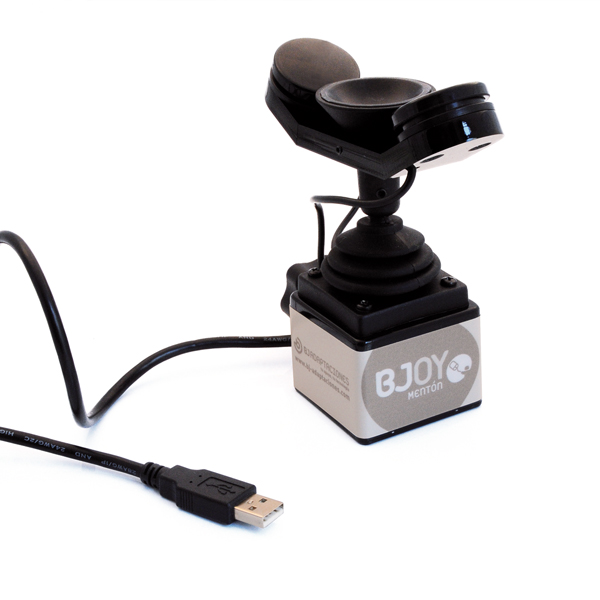
\includegraphics[width=.3\textwidth]{sensory_kinn}
\\
  (c)
\end{tabular}
%
\caption{(a)~Moso® Kinnsteuerung \cite{MOSO}, (b)~Smile Smart Kinnsteuerung \cite{SMILESMART} und (c)~Sensory Kinnsteuerung \cite{SENSORY}.}
\label{fig:kinn}
\end{figure}
\newline \newline
Wie in Abb.~\ref{fig:kinn}(a) zu sehen ist verwendet das Unternehmen moso®%
\footnote{http://www.moso-gmbh.de/}
%
einen Joystick und zwei Tasten für die Interaktion. Um einen angenehmen Umgang zu gewährleisten, ist der Joystick mit einem kleinen weichen Ball ausgestattet. Zwei Tasten sind links und rechts des Joysticks angebracht. Der Joystick kann sich in alle Himmelsrichtungen bewegen und kann so entweder als Mauszeiger, oder zur Steuerung eines Rollstuhls genutzt werden. Die beiden Tasten können als linke und rechte Maustaste verwendet werden \cite{MOSO}.
\newline
Abb.~\ref{fig:kinn}(b) zeigt die Version der Firma Smile Smart Technology%
\footnote{https://smilesmart-tech.com/}
%
. Diese besteht aus einem Mini Rollstuhl Joystick, der auf einer schwenkbaren Halterung montiert ist \cite{SMILESMART}.
\newline
Die Kinnsteuerung des Unternehmens Sensory Guru%
\footnote{http://www.sensoryguru.com/}
%
weist im Vergleich zu den anderen beiden keinen Ball auf. Wie in Abb.~\ref{fig:kinn}(c) dargestellt, weist der Joystick eine Mulde für das Kinn auf. Mit einer Bewegung nach links oder rechts können die beiden äußeren Sensoren aktiviert werden. Das Kinn muss dabei im ständigen Kontakt mit dem Ball bzw. Joystick stehen \cite{SENSORY}. 
\newline
Durch eine stärke Kinnbewegung nach links bzw. rechts oder über zusätzlich angebrachte Tasten an der Steuerung, kann durch ein Menü navigiert werden. Des Weiteren können auch andere Symbole auf einem Bildschirm ausgewählt werden. Durch die Bedienung des Joystickelementes kann der Benutzer beispielsweise die Bewegungen einer Computermaus nachahmen \cite{MOSO} \cite{SENSORY}. 
\newline
Dies kann je nach Ausführung der Steuerung verschieden viele Freiheitsgrade beinhalten. Freiheitsgrade bzw. Degrees of Freedom (DoF) bezeichnen die Bewegungsfreiheit eines Körpers.
\newline \newline
Abb.~\ref{fig:6DoF} zeigt sechs Freiheitsgrade bzw. sechs verschiedene Bewegungsrichtungen \cite{6DoF}:
\begin{itemize}
      \item Hinauf und hinunter (Up and Down)
      \item Links und rechts (Left and Right)
			\item Vorwärts und Rückwärts (Forward and Back)
			\item Kippen entlang der X-Achse (Roll)
      \item Kippen entlang der Y-Achse (Pitch)
			\item Kippen entlang der Z-Achse (Yaw)
\end{itemize}
%
\vspace{\baselineskip}
Bei der Kinnsteuerung von Mosco werden fünf Freiheitsgrade ermöglicht, das bedeutet dass der Joystick in alle Richtungen bewegt und geneigt werden kann, das Kippen entlang der Z-Achse ist allerdings nicht möglich. Bei der Ausführung des Unternehmens Sensory sind nur vier Freiheitsgrade möglich, da der Joystick nicht in Z-Richtung bewegt werden kann. 
Wie stark der Joystick in die bestimmte Richtung gedrückt werden muss, um eine gewisse Bewegung zu erzeugen, kann an den jeweiligen Benutzer angepasst werden, um eine optimale Interaktion zu erreichen.
%
\begin{figure}
\centering
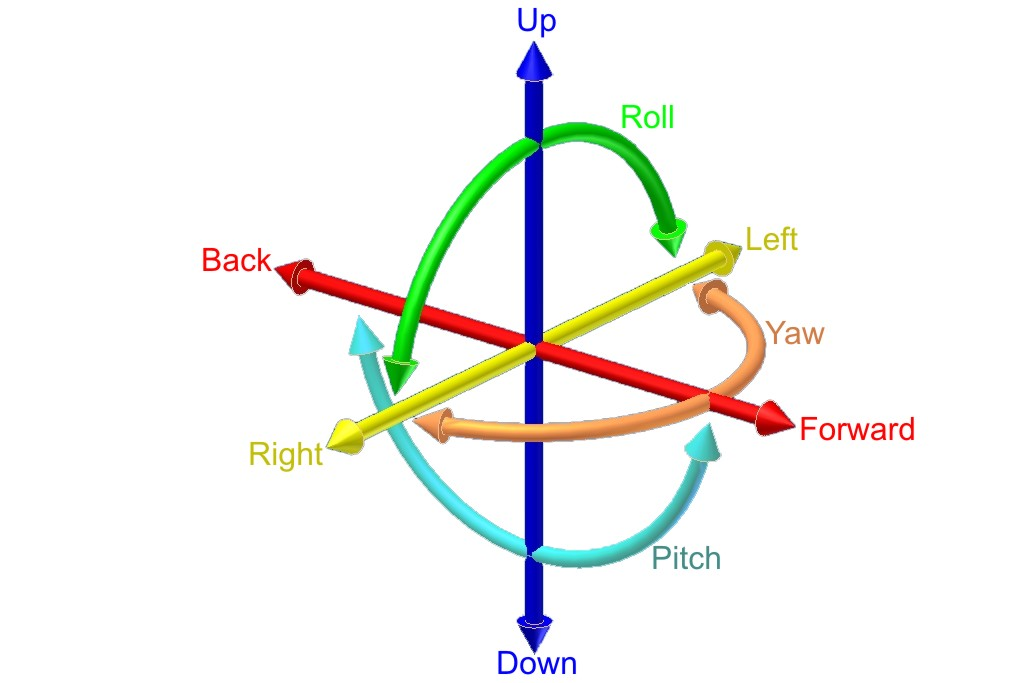
\includegraphics[width=.68\textwidth]{6DoF}
\caption{Sechs Freiheitsgrade \cite{6DoFPic}.}
\label{fig:6DoF}
\end{figure}
%
%

%%%%%%%%% Mundsteuerung %%%%%%%%%
\subsection{Mundsteuerung}

Das Prinzip der Mundsteuerung funktioniert ähnlich wie die Kinnsteuerung. Durch die verschiedenen Interaktionsmöglichkeiten, die durch den Einsatz des Mundes möglich sind, wird versucht, eine Interaktion, beispielsweise mit einem Computer, möglich zu machen.
\newline \newline
Bei der in Abb.~\ref{fig:mund}(a) gezeigten Mundsteuerung handelt es sich um die IntegraMouse Plus, die das Unternehmen LIFEtool%
\footnote{http://www.lifetool.at/startseite/}
%
entwickelt hat. Durch das Bewegen des Mundstückes der IntegraMouse Plus kann die Richtung bzw. der Cursor verändert werden. Zusätzlich zur reinen Steuerung durch eine Geste kann durch Pusten ein Rechtsklick und durch Nippen ein Nippen ein Linksklick erzeugt werden \cite{INTEGRA_VIDEO}.
\newline \newline
Ähnlich wie bei der IntegraMouse Plus wird bei dem mundgesteuerten Gamecontroller der Firma QuadStick%
\footnote{http://www.quadstick.com/}
%
, der in Abb.~\ref{fig:mund}(b) zu sehen ist, ebenfalls Nippen, Pusten und die Bewegungen des Mundes zur Interaktion verwendet. Dieses Modell besitzt allerdings vier Nipp- bzw. Pustsensoren, um einen regulären Gamecontroller besser imitieren zu können. Die drei zusätzlichen Sensoren können individuell angepasst und beispielsweise als Shortcuts für bestimmte Computerspiele verwendet werden. Ein Shortcut bzw. ein Sensor beinhaltet eine Reihenfolge von Klick- und Bewegungsabläufen, die als Kombination dargestellt werden können \cite{QUADSTICK}. In einem gewöhnlichen Computersetting könnten die Shortcuts beispielsweise als Scrollbewegung verwendet werden, die ansonsten durch das hinauf oder hinunterbewegen mit zwei Fingern am Touchpad funktionieren.
\newline \newline
Bei beiden Steuerungen ist vor der Benutzung keine Kalibrierung notwendig. Lediglich muss ein USB-Stick am Computer angeschlossen werden, der die Mundsteuerung per Bluetooth-Verbindung ermöglicht. 

\begin{figure}
\centering\small
\setlength{\tabcolsep}{0mm}	% alle Spaltenränder auf 0mm
\begin{tabular}{c@{\hspace{15mm}}c} % mittlerer Abstand = 12mm
  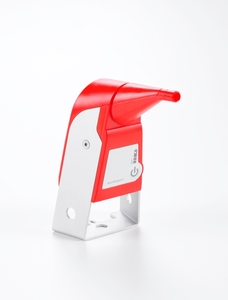
\includegraphics[width=.29\textwidth]{IntegraMouse} &
  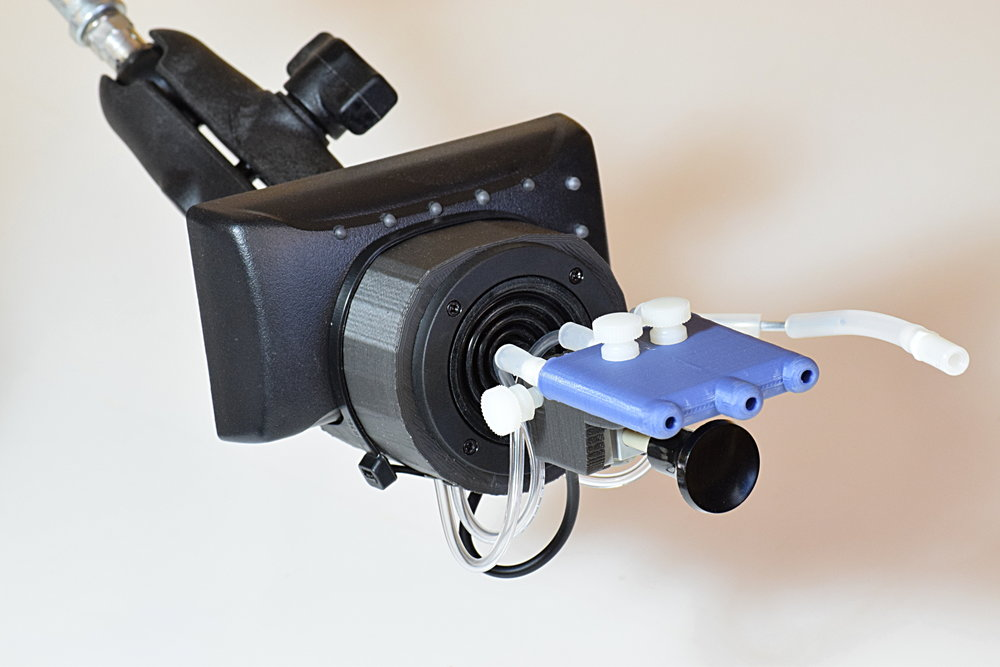
\includegraphics[width=.4\textwidth]{quadstick}
\\
  (a) & (b)
\end{tabular}
%
\caption{(a)~IntegraMouse Plus \cite{INTEGRA} und (b)~QuadStick Gamecontroller \cite{QUADSTICK}}
\label{fig:mund}
\end{figure}

%%%%%%%%% Kopfsteuerung %%%%%%%%%
\subsection{Kopfsteuerung}

Es gibt zwei verschiedene Arten, wie durch den Einsatz des Kopfes mit einem System interagieren werden kann. Zum einen kann eine Kamera verwendet werden, um die Bewegungen des gesamten Gesichtes oder eines bestimmten Teiles davon (z.B. des Mundes) zu verfolgen und diese dann anschließend von einem System in die gewünschten Befehle umzuwandeln. Andererseits kann auch eine Vorrichtung am Kopf befestigt werden und die Interaktion funktioniert durch die Neigungsberechnungen der Sensoren, die Teil der Vorrichtung sind.
\newline \newline
Bei der zweiten Variante könnte beispielsweise ein Stirnband am Kopf befestigt werden, das mit je einem Sensor links und rechts ausgestattet ist. Wird der Kopf in eine Richtung geneigt, wird einer der beiden Sensoren aktiviert. Das Stirnband müsste dafür über Bluetooth oder WLAN mit einem Computer verbunden sein, damit eine Software die Bewegungen bzw. Sensoren erkennen und auswerten kann. Damit das Stirnband benutzt werden kann, müsste es individuell angepasst werden, da die seitliche Neigung des Kopfes je nach Benutzer unterschiedlich ist.
\newline \newline
Bei der optischen Variante werden grundlegend zwei Arten der Kopfsteuerung bzw. der Nachvollziehbarkeit der Bewegungen unterschieden:
\begin{itemize}
      \item Gesichtserkennung
      \item Punkteverfolgung
\end{itemize}
\vspace{\baselineskip}
Bei der Gesichtserkennung wird versucht das Gesicht als Gesamtheit zu erfassen und dieses als Berechnungsgrundlage für die Bewegungen heranzuziehen. Es gibt verschiedene Arten, um die Position des Kopfes zu erkennen. So kann beispielsweise die Hautfarbe dazu verwendet werden. Da diese von Mensch zu Mensch verschieden ist, ist davon abzuraten sie als Erkennungsgrundlage heranzuziehen. Des Weiteren sind bei der Berechnung bzw. Filterung viele Schritte notwendig, was mit großem Rechenaufwand verbunden ist. Daher ist eine Mischung aus der haarähnlichen-Gesichtserkennung und dem Camshift-Gesichtstrackingalgorithmus effizienter.
\newline \newline
Für letztere sind grob drei Schritte notwendig \cite{FaceTracking}:
\begin{itemize}
      \item Als Ausgangslage wird der Unterschied vom Haaransatz zum Gesicht verwendet. Hierbei wir das Gesicht in verschiedene Bereiche aufgeteilt.
			\item Danach wird eine Wahrscheinlichkeitsberechnung durchgeführt, damit erkannt werden kann ob es sich bei den einzelnen Pixeln um den Haaransatz oder das Gesicht handelt.
			\item Abschließend kann auf Grund der Berechnung das Gesicht erkannt werden.
\end{itemize}
\vspace{\baselineskip}
Bei der Punkteverfolgung wird ein bestimmter Teilbereich des Gesichtes fokussiert, der die Bewegungsgrundlage des gesamten Kopfes darstellt. Naizhong und Jing \cite{MouthChinaControl} haben einen Algorithmus entwickelt, der die Mundbewegungen als Grundlage für die Kopfbewegungen verwendet. Dafür wird eine Kamera für den Videoinput verwendet. In der Analyse können die verschiedenen Eingabebefehle unterschieden werden. So ergibt beispielsweise ein Kopfschütteln nach Links einen Linksklick oder ein zweimaliges Kopfschütteln nach Rechts einen rechten Doppelklick \cite{MouthChinaControl}.
\newline \newline
Für den Benutzer gibt es einige Punkte, die vor und während der Interaktion ausschlaggebend für eine optimale Verwendung sind. Ähnlich wie bei der Augensteuerung in Abschnitt ~\ref{cha:Augensteuerung} muss auch hier das System vorab kalibriert werden, um eine reibungslose Interaktion zu ermöglichen. Des Weiteren gilt es zu beachten, dass keine störenden Lichtquellen auf das Gesicht fallen und ein möglichst frontaler Blick in die Kamera erfolgt \cite{MouthChinaControl}.


%%%%%%%%% Fußsteuerung %%%%%%%%%
\subsection{Fußsteuerung}

Es gibt eine Vielzahl an verschiedenen Fußsteuerungen. Manche ähneln dem System der Kinnsteuerung und verwenden einen Joystick, um beispielsweise Mausbewegungen zu erzeugen. Darüber hinaus werden verschiedene Tasten für die Auswahl bestimmter Elemente genutzt. Andere wiederum verwenden einen zusätzlichen Schuh bzw. eine Halterung um den Fuß, um die Fußbewegungen zu messen.
%
%
\begin{figure}
\centering\small
\setlength{\tabcolsep}{0mm}	% alle Spaltenränder auf 0mm
\begin{tabular}{c@{\hspace{0mm}}c} % mittlerer Abstand = 12mm
  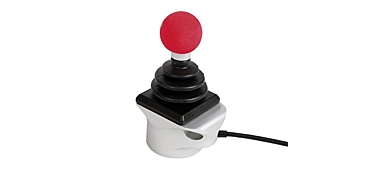
\includegraphics[width=.47\textwidth]{fruewald_joystick} &
  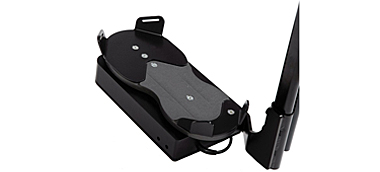
\includegraphics[width=.47\textwidth]{fruehwald_pedal}
\\
  (a) & (b)
\\[7pt]	%vertical extra spacing (4 points)
  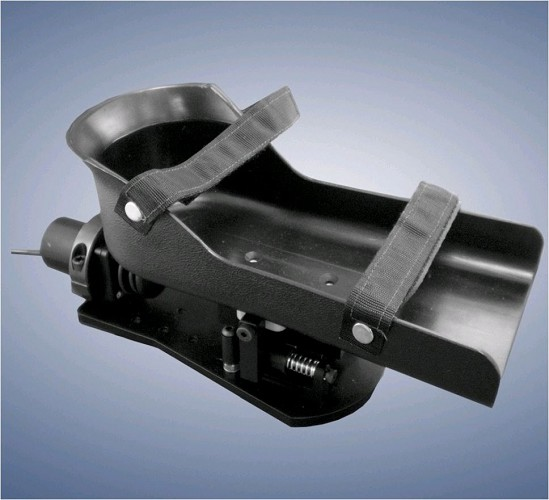
\includegraphics[width=.27\textwidth]{hidrex_pedal}
\\
  (c)
\end{tabular}
%
\caption{(a)~Früwald Joystick \cite{FRUEHWALD}, (b)~Frühwald Fußsteuerung \cite{FRUEHWALD} und (c)~Hidrex Fußsteuerung \cite{HIDREX}.}
\label{fig:foot}
\end{figure}
%
%
\newline \newline
Wie in Abb.~\ref{fig:foot}(a) zu sehen ist, kann ein gewöhnlicher Joystick, der auch mit dem Kinn bedienbar ist, ebenfalls mit dem Fuß bedient werden. Der Benutzer bewegt den Joystick in die gewünschte Richtung und kann damit beispielsweise die Fahrtrichtung eines Rollstuhls oder die Mausbewegung am Computer steuern. Die Fußsteuerung bzw. das Fußpedal (Abb.~\ref{fig:foot}(b)) des Unternehmens Frühwald%
\footnote{https://www.fruehwald.net/}
%
kann durch unterschiedlich starke Druckausübung zur Steuerung verwendet werden \cite{FRUEHWALD}. 
\newline \newline
Bei der in Abb.~\ref{fig:foot}(c) dargestellten Fußsteuerung der Firma Hidrex%
\footnote{http://www.hidrex.de/}%
, handelt es sich um einen Schuhhalter, der als Joystick funktioniert. Die Bedienung ist ähnlich der eines herkömmlichen Joysticks. Der Fuß muss in die gewünschte Richtung gezogen bzw. bewegt werden, um einen Bewegungsablauf nachvollziehen zu können.
%
\newline \newline
Wie die einzelnen Systeme die verschiedenen Gesten in eine Bewegung umwandeln, ist von System zu System verschieden. Häufig findet ein joystickähnliches Element für die Bewegungsrichtung Verwendung. Zusätzliche Tasten helfen bei der Auswahl von gewünschten Symbolen oder Elementen.

%%%%%%%%%%%%%%%%%%%%%%% Muskelsteuerung %%%%%%%%%%%%%%%%%%%%%%%%%%%
\section{Muskelsteuerung}

Bei der Muskelsteuerung wird das Zusammenziehen eines Muskels oder bestimmter Muskelpartien verwendet, um so mit einem Computer interagieren zu können.
\newline \newline
Der Großteil der Muskelsteuerungssysteme nützt zur Messung der Signale das Prinzip der Elektromyografie (EMG). Bei einer EMG-Schnittstelle handelt es sich um die Messung der Muskelkontraktionen. Zusätzlich muss diese Messung mit einer Software für die gewünschten Interaktion verknüpft werden. Die Voraussetzung an den Benutzer besteht lediglich darin, die ausgewählten Muskelpartien selbstständig anzuspannen bzw. zu aktivieren. Im Zusammenhang mit der Muskelsteuerung kommt die Oberflächenelektromyografie (sEMG, englisch für Surface Electromyography) zum Einsatz. Hierbei werden die Elektroden, die für die Messung der Signale ausschlaggebend sind, an der Hautoberfläche angebracht. Mit Hilfe der Elektroden können die myoelektrischen Signale, die die Muskeln produzieren, gemessen und in einem späteren Schritt als bestimmte Interaktion interpretiert werden \cite{EmgDefinition}.
\newline \newline
Abb.~\ref{fig:MyoAblaufOhr} zeigt die einzelnen Schritte, die das Signal im System durchläuft, um am Ende die Interaktion mit einem Computer zu ermöglichen. In der Studie von Barszap, Skavhaug und Joshi \cite{MyoOhr} werden zwei Frequenzbänder verwendet, um eine X- und Y- Richtung des Mauszeigers zu ermöglichen. Zieht sich der Muskel zusammen, so werden alle messbaren Signale erfasst und die relevanten herausgefiltert. Anschließend werden die Signale in zwei Partien aufgeteilt und durch zwei separate Bandpassfilter geschickt. \newline
Dadurch werden die gewünschten Signale bzw. Frequenzen erneut gefiltert und angepasst. Danach werden die beiden Signale in einen Wert zwischen 0 und 100 umgerechnet, der die Ausprägungsstärke in Prozent der jeweiligen Koordinate repräsentiert \cite{MyoOhr}.
\newline \newline
Damit ein Benutzer durch den Einsatz von myoelektrischen Signalen mit einem Computer interagieren kann, müssen zu Beginn die richtigen Positionen für die Anbringung der Elektroden gefunden werden.  
\newline \newline 
Es gibt verschiedene Ansätze, wie die Kalibrierung im Detail aussehen kann. Folgendes Beispiel bezieht sich auf eine Studie von Vernon und Joshi \cite{MyoTraining}.
%
%
\begin{figure}
\centering
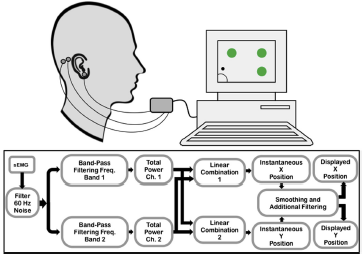
\includegraphics[width=.5\textwidth]{MyoAblaufOhr}
\caption{EMG Signalverarbeitung \cite{MyoOhr}}
\label{fig:MyoAblaufOhr}
\end{figure}
%
%
\begin{figure}
\centering\small
\setlength{\tabcolsep}{0mm}	% alle Spaltenränder auf 0mm
\begin{tabular}{c@{\hspace{15mm}}c} % mittlerer Abstand = 12mm
  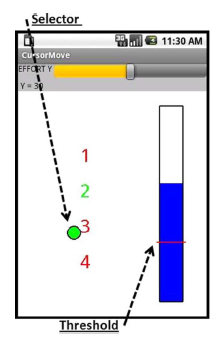
\includegraphics[width=.28\textwidth]{MyoTraining1} &
  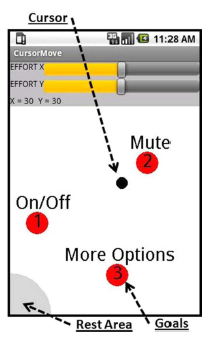
\includegraphics[width=.28\textwidth]{MyoTraining2}
\\
  (a) & (b)
\end{tabular}
%
\caption{Trainingsoberflächen: \newline
1D-Steuerung \cite{MyoTraining}~(a) und 2D-Steuerung \cite{MyoTraining}~(b)}
\label{fig:MyoTraining}
\end{figure}
%
%
\newline
Die Elektroden werden an der vermuteten Stelle der zu messenden Muskeln angebracht und mit dem Computer verbunden. Auf dem Bildschirm ist das aktuelle sEMG-Signal zu sehen. Beinhaltet das Signal viele Störfaktoren, das sog. Rauschen, müssen die Elektroden gereinigt oder neu positioniert werden. Ist die optimale Position gefunden worden, muss das System an die individuellen Muskelkontraktionen des Anwenders angepasst werden. Bei diesem Schritt muss der Benutzer die ausgewählten Muskeln über einen Zeitraum von einigen Sekunden so fest wie möglich anspannen, um die maximale Frequenz bzw. Leistung erfassen zu können. Als nächstes werden beim Benutzer zwei verschiedene Testphasen durchgeführt. Der erste Test (Abb.~\ref{fig:MyoTraining}(a)) dient dazu, ein Bewusstsein zu entwickeln, wann und wie stark der gewünschte Muskel angespannt werden soll. Der grüne Punkt auf dem Display bewegt sich je nach Anspannung durch die verschiedenen Stufen und soll auch durch Entspannen wieder zur Ausgangslage gebracht werden. Bei dem zweiten Test, der in Abb.~\ref{fig:MyoTraining}(b) dargestellt ist, handelt es sich um eine zweidimensionale Überprüfung. Hier soll der Cursor in X- und Y-Richtung bewegt werden. Dies geschieht ebenfalls durch An- und Entspannung der einzelnen Muskeln. Beide Versuche bauen auf dem Trial und Error Prinzip auf. Der Benutzer muss also durch mehrere Versuche zur richtigen bzw. besten Lösung kommen. Ist der Anwender mit beiden Trainings vertraut, kann mit der gewünschten Interaktion mit dem Computer begonnen werden. Diese ist auf dem selben Prinzip aufgebaut, allerdings gibt es unterschiedliche Oberflächen, Anordnungen der Elemente und Unterscheidungen in der Aufgabenstellung selbst \cite{MyoTraining}.
\newline \newline
Abb.~\ref{fig:MyoBand} zeigt das Armband des Unternehmens Myo%
\footnote{https://www.myo.com/}
%
. Dieses verwendet die myoelektrischen Signale des Armes, um durch verschiedene Gesten mit dem Computer interagieren zu können. Zu den fünf vordefinierten Gesten zählen z.B. das Bilden einer Faust oder Wischgesten. Es können aber auch eigene Gesten definiert bzw. programmiert werden. Zum einen können die vordefinierten Gesten durch die Einberechnung von Armbewegungen erweitert werden, zum anderen gibt es die Möglichkeit neue Gesten zu erstellen, da der Zugriff auf die rohen EMG-Daten möglich ist \cite{myoBand2}.%
\newline \newline \newline 
Damit ein Computer mit Hilfe von Muskelkontraktionen gesteuert werden kann, ist ein aufwendiger und gut überlegter Algorithmus notwendig, um die erfassten Signale in das gewünschte Ergebnis zu transferieren. Vor der Interaktion müssen wie beschrieben einige Schritte durchlaufen werden, um das System an das Individuum anzupassen und um ein Bewusstsein für die Muskelsteuerung zu erlangen.
%
%
\begin{figure}
\centering
\includegraphics[width=.3\textwidth]{MyoBand}
\caption{Myo Armband \cite{myoBand}.}
\label{fig:MyoBand}
\end{figure}
%
%

%%%%%%%%%%%%%%%%%%%%%%% Gehirnaktiviät %%%%%%%%%%%%%%%%%%%%%%%%%%%
\section{Steuerung durch Gehirnaktivität}

Dieser Abschnitt beschäftigt sich mit der Schnittstelle zwischen dem Gehirn und dem Computer. In der Literatur wird in diesem Zusammenhang von Brain-Computer-Interface (BCI) gesprochen. Ziel ist es, eine direkte Verbindung der beiden Komponenten für eine Interaktion herzustellen. Das BCI liest die Wellen, die vom Gehirn an den verschiedensten Stellen produziert werden ein und übersetzt diese Signale in Befehle, damit mit einem Computer interagiert werden kann \cite{BRAIN}.
\newline \newline
Es gibt verschiedene Aufnahmetechniken von BCIs:
\begin{itemize}
      \item Invasiv
      \item Teilweise invasiv
			\item Nicht invasiv
\end{itemize}
\vspace{\baselineskip}
Invasive Gehirn-Computer-Schnittstellen werden direkt im menschlichen Gehirn durch eine Operation eingesetzt. Es können hier einzelne oder mehrere Einheiten in verschiedenen Bereichen des Gehirns platziert und anschließend angesprochen werden. Diese Systeme weisen die höchste Qualität auf, bringen aber durch die Operation gewisse Risiken mit sich.
Bei teilweise invasiven BCI-Systemen werden die Einheiten nicht direkt in den Gehirnzellen sondern im Schädel eingesetzt, allerdings können sie daher die Signale etwas schlechter empfangen. Bei nicht invasiven Systemen handelt es sich um die sicherste und kostengünstigste Variante auf Kosten von schwächerem Gehirnsignalempfang. Die Signale werden über Elektroden empfangen, die am Kopf befestigt werden. Für diese Technik werden meist mit Hilfe eines Elektroenzephalografen (EEG) die neuronalen Wellen des Gehirns gemessen \cite{BRAIN}.
\newline \newline 
Die neuronale Aktivität des Gehirns ist ausschlaggebend für die Messung. Daher ist es wichtig, die verschiedenen Signale, die ein EEG misst, kurz darzustellen \cite{BRAIN}:
\begin{itemize}
      \item Delta Signal: Hierbei handelt es sich um die langsamsten Wellen mit einer Frequenz zwischen 0.5 und 3.5 Hz, die während des Schlafens oder im komatösen Zustand auftreten.
      \item Theta Signal: Es handelt sich hierbei um Wellen, die beispielsweise während des Träumens vorkommen. Die Frequenzen werden in einem Bereich zwischen 3.5 und 7.5 Hz gemessen.
			\item Alpha Signal: Dies sind langsamere Wellen, die beim Entspannen auftreten (Frequenzen zwischen 7.5 und 12 Hz).
			\item Beta Signal: Diese Wellen sind oft mit Anstrengung, wie beispielsweise des Lösens einer mathematischen Aufgabe, verbunden und liegen in einem Bereich zwischen 12 und 30 Hz.
      \item Gamma Signal: Je größer hier die Amplitude ist, desto mehr Stress, Angst oder Panik erlebt die Personen (alle Frequenzen ab 31 Hz).
\end{itemize}
\vspace{\baselineskip}
Je nach Anwendungsbereich können verschiedene Signale verwendet werden. Für eine Interaktion mit einer Person, die sich nicht in einem komaähnlichen Zustand befindet, sind alle Signale ab einer Stärke von 3.5 Hz relevant.
\newline \newline
%
%
\begin{figure}
\centering
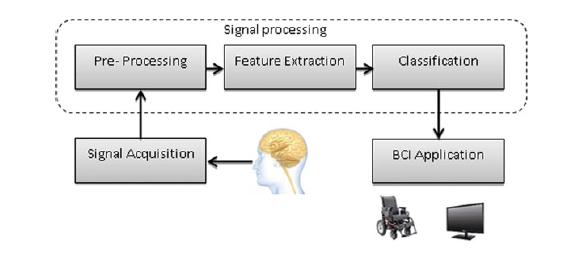
\includegraphics[width=.9\textwidth]{BCI}
\caption{BCI Signalverarbeitung \cite{BRAIN}.}
\label{fig:BCI}
\end{figure}
%
%
Für den gesamte Ablauf, der nötig ist, um eine Gehirn-Computer-Schnittstelle zu erstellen sind, wie in Abb.~\ref{fig:BCI} veranschaulicht, sind grob drei Schritte notwendig \cite{BRAIN}:
\begin{itemize}
      \item Signalerfassung: Im ersten Schritt werden die elektrischen Signale von der Kopfhaut oder der Oberfläche des Gehirns erfasst.
      \item Signalverarbeitung: Da die diese Signale in der Regel sehr schwach sind, werden sie als nächstes verstärkt und von Störvariablen gereinigt. Danach durchlaufen die Signale einen Übersetzungsalgorithmus, damit die Absichten des Benutzers erkannt werden können.
			\item Signalinterpretation: Im letzten Schritt müssen die Daten von einem Programm bzw. einer Software so interpretiert werden, damit diese für eine Computerinteraktion verwendet werden können.
\end{itemize}
%
%
\vspace{\baselineskip}
\vspace{\baselineskip}
\vspace{\baselineskip}
Um als Benutzer einen Computer mit Hilfe von Gehirnaktivität steuern zu können, muss das System vor der Interaktion individuell angepasst werden. Als mögliche Kalibrierungsmethode kann ein Mauszeiger gedanklich mitverfolgt werden, während dieser sich bewegt. Der Benutzer soll sich hierbei vorstellen, er würde die Bewegung mit der Hand oder dem Arm ausführen. Je nach Person zeigt sich eine Anstrengung in dem motorischen Teil des Gehirns unterschiedlich stark und das System wird dahingehend angepasst. Im nächsten Schritt wird erneut ein Mauszeiger gedanklich mitverfolgt. Allerdings erscheint ein zweiter Cursor, der auf Grundlage der bereits erhobenen Daten den momentanen Stand aufzeigt. Diese zwei Schritte werden mehrmals durchgeführt, um ein optimales Ergebnis zu erzielen. Neben der Mausbewegung kann auch ein Mausklick simuliert werden. Die Auswahl eines Menüpunktes kann beispielsweise dann so funktionieren, dass ein Menüpunkt hervorgehoben wird. Hat der Anwender sich für einen bestimmten entschieden, muss er sich besonders darauf konzentrieren bzw. die Gehirnbereiche müssen eine erhöhte Aktivität vorweisen \cite{BrainInt}.
\newline
Es muss darüber hinaus nicht nur der Benutzer an das System angepasst werden, sondern auch umgekehrt. Bei jeder Interaktion kann das System die Eigenheiten des Individuums besser erfassen, bessert Fehler aus und kann sich durch das ständige Mitlernen verbessern. 
\newline \newline
Die Interaktion mit Hilfe der Messung der Gehirnaktivität ist im Gegensatz zu den zuvor beschrieben Methoden eine komplexere und aufwendigere Eingabemethode. Auch die Interaktion ist mit viel Aufwand hinsichtlich der Kalibrierung und des Trainings des Systems verbunden.

\chapter{Ausgabemethoden}
\label{cha:Ausgabe}

Im Kapitel~\ref{cha:Eingabe} wurden alternative Eingabemethoden zur Interaktion Hands-Free näher erläutert. Dieses Kapitel befasst sich mit Ausgabemethoden, die aber nicht zwingend an bestimmte Eingabemethoden gebunden sind. So gibt es nicht nur bei Systemen, die über die Sprache gesteuert werden, ein akustisches Feedback, sondern auch bei Systemen, die beispielsweise über die Augen oder den Mund gesteuert werden. 


%%%%%%%%%%%%%%%%%%%%%%% Auditiv %%%%%%%%%%%%%%%%%%%%%%%%%%%
\section{Auditive Ausgabe}

Eine mögliche Form, wie ein Computer Feedback geben kann, geschieht durch eine auditive Ausgabe. Dies kann entweder durch ein Geräusch, ein Signal oder durch die Sprachausgabe funktionieren.
\newline \newline
Eine Möglichkeit auditives Feedback zu erhalten sind vom Computer erzeugte Signale oder bestimmte Geräusche. Bei diesen Signalen bzw. Geräuschen handelt es sich beispielsweise um einen hohen angenehmen Ton bei korrektem Verhalten oder um einen dumpfen unangenehmen Ton bei einer Fehlereingabe. Hierbei handelt es sich aber nicht ausschließlich um Töne, sondern auch Klick-Geräusche können als Ausgabe fungieren. So gibt ein Lautsprecher bei einer Fußgängerampel beispielsweise ein kontinuierliches Klick-Geräusch von sich, wenn es rot ist. Schaltet die Ampel auf grün verdoppeltet sich die Geschwindigkeit des Geräusches.
\newline \newline
Weitaus komplexer ist allerdings die Sprachausgabe. Während bei der Spracheingabe die gesprochene Sprache von einem System in einen Befehl umgewandelt wird, gibt bei der Sprachausgabe der Computer die Informationen in Form von Sprache aus. Da die Sprachausgabe von Menschen gehört und automatisch bewertet wird, ist es wichtig, dass die Sprache von hoher Qualität ist, also möglichst real erscheint. 
\newline
%abbildung 1
\begin{figure}
\centering
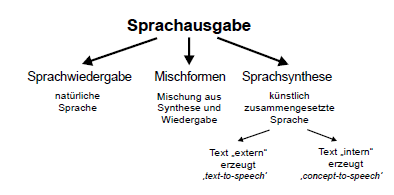
\includegraphics[width=.7\textwidth]{sprachausgabe_overview}
\caption{Unterteilung der Sprachausgabe \cite{FellbaumSprache}.}
\label{fig:SprachausgabeOverview}
\end{figure}
%	
Wie in Abb.~\ref{fig:SprachausgabeOverview} dargestellt gibt es zwei unterschiedliche Ansätze, wie der Computer den Text in Sprache umwandeln kann:
\begin{itemize}
      \item Sprachwiedergabe
      \item Sprachsynthese
\end{itemize}
\vspace{\baselineskip}
\vspace{\baselineskip}
%SPRACHWIEDERGABE
Bei der Sprachwiedergabe werden Sprachsignale ausgegeben, die zuvor aufgenommen und abgespeichert worden sind. Der Umfang an möglichen akustischen Meldungen also an Wörtern ist aus diesem Grund an die Anzahl der Aufnahmen gebunden und daher begrenzt. Da die Signale bzw. Wörter von einer realen Person eingesprochen wurden, weißt diese Methode eine sehr hohen Sprachqualität auf \cite{KaufmannPfisterSprache}.
\newline \newline
Es gibt unterschiedliche Methoden bzw. Verfahren, wie die Sprachwiedergabe im Detail funktioniert. Zusammenfassend werden die Wörter zu Beginn von einer Person eingesprochen, bearbeitet und abgespeichert. Die einzelnen Sprachelemente werden anschließend adressiert, sodass sie vom System später leicht gefunden werden können. Wenn der Computer nun einen Text vorlesen soll, wird im System anhand der gespeicherten Adressen die einzelnen Wörter bzw. Phrasen herausgesucht und verwendet \cite{FellbaumSprache}.
\newline \newline
%SPRACHSYNTHESE
Im Gegensatz zur Sprachwiedergabe wird bei der Sprachsynthese das Ziel verfolgt alle möglichen Wortkombinationen in ein Sprachsignal umwandeln zu können. Da die Grundlage für die Wörter bzw. Ausgabe nicht von einer Person eingesprochen werden, sondern die einzelnen Wörter mit ihrer Betonung künstlich erzeugt werden müssen, sinkt dadurch die Sprachqualität und das Endergebnis gleicht oft mehr einer Computerstimme als der einer menschlichen. 
\newline \newline
Bei der Sprachsynthese werden Silben aus verschiedenen Wörtern einzeln abgespeichert und so alle beliebigen Kombinationen zusammengesetzt. Im Anschluss werden Betonungen, Lautstärke und Geschwindigkeit hinzugefügt bzw. angepasst. Bei der sogenannten textgesteuerte Sprachsynthese (‚text-to-speech‘) ist dem System der eigentliche Inhalt des Textes nicht bekannt. Es können aber nicht nur einzelne Sätze bzw. ganze Texte verarbeitet werden, sondern auch Konzepte können vom System in Signale umgewandelt werden (,concept-to-speech'). Hier kann das System einen Text eigenständig kreieren, wenn das Konzept bzw. der Inhalt bekannt ist \cite{FellbaumSprache}.
\newline \newline
%zitat Fellbaum
Laut Fellbaum \cite{FellbaumSprache} besteht die größte Herausforderung der Sprachsynthese darin, die Stimme noch natürlicher und nicht roboterähnlich wirken zu lassen. Daher sind Mischformen zwischen Sprachwiedergabe und Sprachsynthese in der Praxis üblich. 


%%%%%%%%%%%%%%%%%%%%%%% Haptisch %%%%%%%%%%%%%%%%%%%%%%%%%%%
\section{Haptische Ausgabe}
%TODO what to write here
%definition haptik
Haptische Ausgabe beinhaltet jene Arten von Feedback bei der etwas durch den menschlichen Tastsinn wahrgenommen werden kann. Hierbei gibt es verschiedene Arten:
%
%
\begin{itemize}
      \item Thermales Feedback (Wärme)
      \item Vibration
			\item Feedback durch ein haptisches Steuerungselement
\end{itemize}
\vspace{\baselineskip}
%
%
Bei thermaler Ausgabe handelt es sich um Feedback in Form von Wärme. Der Computer bzw. das Gerät mit dem interagiert wird erhitzt sich auf eine vordefinierte Temperatur und kühlt sich wieder ab. Lee & Lim \cite{LeeLim} haben festgestellt dass warme Temperaturen mit etwas positiven und kalte Temperaturen mit etwas Negativem verbunden werden. Des Weiteren konnte die Teilnehmer eine Abstufung der Wärmeunterschiede feststellen, die über eine strikte Trennung von warm oder kalt überschreiten. Die Veränderungen von warm auf kalt oder umgekehrt sollen nicht zu plötzlich geschehen, da dies ein Unwohlbefinden bei der Interaktion auslöst \cite{LeeLim}. \newline
Laut Jones & Berri \cite{JonesBerris} soll sich das Ausgabegeräte um max. 20°C/sek abkühlen und um max. 10°C/sek aufwärmen. Auch sollte ein maximaler Unterschied von 20°C nicht überschritten werden.
\newline \newline
Haptische Ausgabe kann auch in Form von Vibration erfolgen. Die Vibration kann sich in ihrer Intensität und Dauer unterscheiden. Diese Art von Feedback kann unter anderem zur Bestätigung einer Eingabe erfolgen \cite{Vibration}. Will ein Benutzer beispielsweise auf einer virtuellen Tastatur einen Buchstaben auswählen, kann bei Erfolg eine leichte Vibration durch ein Armband o.ä. erfolgen.
\newline \newline
%% TODO Haptisches Stuerelement%%
Neben der thermalen Ausgabe und der Ausgabe durch Vibration kann das Feedback auch über das Eingabeelement erfolgen. Handelt es sich bei dem Eingabegerät um einen Joystick kann die Ausgabe durch verschiedene Vibrationsmuster, aber auch durch eine Gegenbewegung seitens des Joysticks in X-, Y- oder Z-Richtung erfolgen, je nachdem wie viele Freiheitsgrade das Eingabegerät erlaubt (vgl. Abschnitt ~\ref{cha:Kinnsteuerung}) \cite{an2002haptic}. 
\newline \newline
Es gibt unterschiedliche Möglichkeiten, wie haptische Ausgabe geschehen kann. Zur Bestätigung einer Eingabe ist ein Feedback zu Vibration meist üblich. Soll ein möglichst realistisches Feedback bzw. eine Interaktion mit dem System gewährleistet werden ist darüber hinaus Feedback vom Eingabeelement durch Bewegungsrichtung empfehlenswert.  
\newpage
%%%%%%%%%%%%%%%%%%%%%%% Visuell %%%%%%%%%%%%%%%%%%%%%%%%%%%
\section{Visuelle Ausgabe}
%TODO what to write here
Um Informationen visuell darzustellen und diese als Ausgabe des Systems zu nutzten, sind ein oder mehrere Displays oder Projektoren notwendig. Die Ausgabe kann entweder auf dem selben Bildschirm wie die Eingabe zu sehen sein, oder auf einem separaten Bildschirm.
\newline \newline
Es gibt sehr viele unterschiedliche Arten, in welcher Form und Ausprägung visuelle Ausgabe erfolgen kann. Dies beginnt bei der simplen Ausgabe eines Feldbacktextes. Wird eine bestimmte Interaktion richtig oder falsch ausgeführt, kann daraufhin ein Text bzw. ein Wort erscheinen, dass den Erfolg bzw. Misserfolg mitteilt. Des Weiteren können auch Bilder oder andere Mediaelemente in einem ähnlichen Kontext aufscheinen. Bei der bloßen Unterscheidung zwischen korrekt und inkorrekt können beispielsweise auch ein grünes Häkchen bzw. ein rotes Kreuz angezeigt werden. Visuelle Ausgabe kann aber nicht nur über unterschiedliche Symbole erfolgen, sondern auch die bloße Änderung der Farbe eines Elementes kann ausschlaggebend für dessen Zustand sein.
\newline \newline
Abb.~\ref{fig:MyoTraining}(a) beschreibt einen Kalibrierungsschritt vor der Verwendung eines Systems, dass durch die Muskelkontraktionen gesteuert werden kann. Hier gibt der Computer laufend visuelles Feedback über den aktuellen Zustand bzw. die Anspannung der Muskeln.
\newline \newline
Bei dem in Abschnitt ~ref{Augensteuerung} erwähnten Augensteuerungssystem des Unternehmens %
\footnote{http://humanelektronik.de/}
%
kann eine virtuelle Tastatur mit Hilfe der Augen bedient werden. Wir ein Buchstabe über einen längeren Zeitraum fokussiert, wird dieser auch ausgewählt. Während der Fixation erscheint eine Sanduhr, die dem Benutzer mitteilt wie lange der gewünschte Buchstabe noch fixiert werden muss \cite{SEETECH}. 
%
\newline \newline
Zusammengefasst kann gesagt werden, dass es sehr viele verschiedene Möglichkeiten gibt, wie ein Computer bzw. das Interaktionsgerät selbst visuell Feedback geben kann. Je nach Anwendungsfall (bloße richtig oder falsch Unterscheidung oder komplexere Ausgabe) können Texte, Symbole, Farben oder auch Kombinationen ausgewählt werden.
%
%
%
\newline \newline \newline
Alle beschriebenen Ausgabemethoden können einem menschlichen Sinn zugeordnet werden (auditive Ausgabe dem Hörsinn, haptische Ausgabe dem Tastsinn und visuelle Ausgabe dem Sehsinn). Aus diesem Grund ist es hier erwähnenswert, dass es Ausgabegeräte gibt die dem Geschmackssinn und dem Geruchssinn zugeordnet werden können. Allerdings kommen diese in der Praxis nur vereinzelt zum Einsatz und sind daher in diesem Zuge dieser Arbeit nur nennenswert relevant. 



\chapter{Gegenüberstellung der Methoden}
\label{cha:Vergleich}

In Kapitel ~\ref{cha:Ausgabe} wurden die verschiedenen Eingabemethoden näher erläutert. Dieses Kapitel beschreibt, welche Vor- und Nachteile, gesonderte Rahmenbedingungen und welche Einsatzgebiete es zu den einzelnen Methoden gibt. Da der Fokus dieser Arbeit auf der Steuerung von Systemen liegt, wird in diesem Kapitel auf die verschiedenen Ausgabemethoden nicht eingegangen.

\section{Fördernde und hemmende Faktoren}
%
Jede einzelne Eingabemethode weist gewisse Pro- und Kontraseiten auf. Für einen Vergleich wurden verschiedene Kriterien definiert. Tab.~\ref{tab:matrixObj} zeigt die objektiven Kriterien, Tab.~\ref{tab:matrixSubj} stellt die subjektiven Kriterien dar.
\newline \newline
Der erste Vergleichsfaktor, der in Tab.~\ref{tab:matrixObj} dargestellt ist, bezieht sich auf die Kosten. Bei der Sprachsteuerung gibt es verschiedene Sprachassistenten, wie \zB Siri%
\footnote{https://www.apple.com/ios/siri/}
%
 oder Cortana%
\footnote{https://support.microsoft.com/en-us/help/17214}
%
 , mit denen ein Computer zum Teil mit Hilfe der Sprache gesteuert werden kann. Die Programme an sich sind kostenlos, wenn der Benutzer über das entsprechende Gerät verfügt (iPhone etc. oder Computer mit Windows10).
Wie in Abschnitt ~\ref{cha:Augensteuerung} erklärt, werden für die Augensteuerung sowohl ein Eye-Tracking-System, als auch eine Software benötigt. Exklusive der Kosten für die Software belaufen sich die in Abb.~\ref{fig:Tobii}(a) dargestellten Tobii Pro Glasses 2 auf rund 13.500€ \cite{TobiiCosts}. Allerdings kann auch eine günstigere Variante implementiert werden. Hierbei benötigt man zwei Webcams (ca. 100€) und eine Open Source Software für die Blickerkennung und Steuerung. Kinn- und Mundsteuerungen kosten zwischen 400€ und 2000€ \cite{SENSORY} \cite{INTEGRA}. Das Myo-Armband als Referenz für die Muskelsteuerung beläuft sich auf ca. 250€, wobei komplexere Systeme wesentlich teurer sind \cite{myoBand}. Das in Abb.~\ref{fig:epoc} dargestellte EPOC+, das dem Benutzer ermöglicht mit einem System mit Hilfe von Gehirnaktivität zu interagieren, kostet rund 720€.
\newline \newline \newline \newline \newline
Die meisten System weisen keine räumliche Einschränkung auf und sie sind daher nicht an ein gewisses Setting gebunden. Bei der Benutzung einer Augensteuerung ist allerdings darauf zu achten, dass keine störenden Lichtquellen die Kamera bzw. die Interaktion behindern. Des weiteren ist ein Benutzer bei der Verwendung von Systemen, die durch die Gehirn- oder Muskelaktivität gesteuert werden, oft an die notwendigen Geräte und somit an gewisse Räumlichkeiten gebunden.
\newline \newline
Die Größe und das Gewicht der Systeme richten sich immer nach den Interaktionsgeräten der jeweiligen Eingabemethode. Für die Augensteuerung können beispielsweise die Geräte, die in Abb.~\ref{fig:Tobii} dargestellt sind, verwendet werden. Hier bewegt sich die Spanne von 312 g für Tobii Pro Glasses 2 bis zu einem Gesamtgewicht von 8.9 kg für die Eye-Tracker-Einheit und den Monitor des Tobii Pro Spectrum. Die Elektroden an sich, die die Basis für die Muskelsteuerung und die Steuerung mit Hilfe von Gehirnaktivität darstellen, sind an sich sehr klein und haben kaum ein Gewicht. Das Myo-Armband, das hier als Beispiel angeführt wird, ist nur 11,9 x 7,4 x 10,4 cm groß und 254 g schwer. Während das EPOC+ des Unternehmens Emotiv mit 23 x 38 x 38 cm und 540 g mehr als doppelt so groß und doppelt so schwer ist.
\newline \newline
Wie zu Beginn schon erwähnt, werden in Tab.~\ref{tab:matrixSubj} subjektive Faktoren als Vergleich der einzelnen Eingabemethoden verwendet.
\newline \newline
Die Dauer, wie lange ein Benutzer mit einem Computer interagieren kann, ist von System zu System sehr unterschiedlich. Da die Sprachsteuerung und die\linebreak Gestensteuerung nur eine geringe kognitive und körperliche Anstrengung erfordern, gibt es bei der Benutzungsdauer kaum Einschränkungen. Im Gegensatz dazu findet man bei der Augensteuerung eine hohe körperliche Anstrengung. Sie sollte daher nicht zu lange eingesetzt werden, damit die Augen langfristig nicht geschädigt werden. Ähnlich wie bei der gewöhnlichen Benutzung eines Computers sollte alle 20 Minuten eine Pause eingelegt werden \cite{20Methode}. Das Benutzen einer Steuerung, die durch Muskeln oder durch Gehirnaktivität funktionieren, ist mit hoher kognitiven Anstrengung verbunden. Zusätzlich erfordert das An- und Entspannen der Muskelpartien intensiven körperlichen Einsatz. Aus diesen Gründen ist die Interaktionsdauer der beiden Methoden sehr beschränkt. Daher muss während der Interaktion regelmäßig überprüft werden, ob zum gegebenen Zeitpunkt eine Überanstrengung erfolgt. Ist dies der Fall, sollte eine Pause eingelegt werden, um den beanspruchten Partien eine Erholungsphase zu ermöglichen.
\newline \newline
Wie lange mit einem System interagiert werden kann, hängt unter anderem von der kognitiven und körperlichen Anstrengung ab. Elisa Mira Holz u.a \cite{holz2013brain} entwickelten ein BCI-Prototypen, mit dem es möglich ist mit Hilfe von Gehirnaktivität mit einem Computerspiel zu interagieren. Nach der Interaktion mit dem Prototypen wurde eine Evaluation zur Einschätzung der subjektive Arbeitsbelastung nach dem NASA-TLX-Fragebogen durchgeführt. Festgestellt wurde, dass nur eine geringe körperliche, jedoch aber eine hohe kognitive Anstrengung besteht. Alle anderen Eingabemethoden wurden anhand der Ergebnisse dieser Studie abgeleitet. Die Steuerung durch Muskelaktivität erfordert eine hohe körperliche Anstrengung, da das Muskelan- und entspannen eine hohe Beanspruchung darstellt. Auch die kognitive Anstrengung ist hier sehr hoch, weil sich der Benutzer zum einen sehr konzentrieren muss, um die Muskeln richtig einsetzten zu können, zum anderen ist diese Interaktionsart hinsichtlich der Bedienbarkeit gewöhnungsbedürftig. Im Vergleich zur kognitiven Anstrengung bei der Steuerung mit Hilfe von\linebreak Gehirnsteuerung, gibt es bei den restlichen Eingabemethoden nur eine geringe Belastung. Einen Ausnahmefall stellt die Augensteuerung dar. Da die Augen ein sehr empfindliches Sinnesorgan sind und die Interaktionsdauer beschränkt ist, wird hier eine hohe körperliche Anstrengung angeführt.
\newline \newline
Weil das Sprechen eine sehr natürliche Form der Kommunikation ist, ist auch die Interaktion mit einem Gerät intuitiv. Ähnliches kann über die Gestensteuerung gesagt werden, da das Bewegen des Joysticks in die einzelnen Richtungen sehr einfach und intuitiv ist. Gewöhnungsbedürftiger für den Benutzer ist die Augensteuerung, da er sich wesentlich mehr konzentrieren und stets den Bildschirm fokussieren muss. Auch die Muskelsteuerung und die Steuerung mit Hilfe von Gehirnaktivität sind gewöhnungsbedürftig, da diese Interaktionsformen keine vertraute Art der Kommunikation darstellen und mit hoher kognitiven Anstrengung verbunden sind.
\newline \newline
Bevor ein Benutzer mit einem System interagieren kann, muss ein Gerät oft individuell angepasst (kalibriert) werden. Dies ist bei allen beschriebenen Eingabemethoden, ausschließlich der Gestensteuerung, der Fall. Bei der Sprachsteuerung ist die Kalibrierung von System zu System verschieden, allerdings nur mit einem sehr geringen Zeitaufwand verbunden. Da die Verwendung einer Muskelsteuerung oder einer Steuerung durch die Gehirnaktivität durch Trial und Error geprägt ist, erfordert auch die Kalibrierung zu Beginn und vor jeder Benutzung einen größeren Aufwand.
\newline \newline
Für die Benutzung jeder der verschiedenen Eingabemethoden gelten die selben Grundvoraussetzungen. Der Benutzer muss eine eigenständige Kontrolle über das jeweilige Eingabemittel (Sprache, Muskelanspannung, Augenbewegungen etc.) besitzen, damit eine Interaktion möglich ist. Zusätzlich gibt es Faktoren, die von Methode zu Methode unterschiedlich sind. So ist bei der Sprachsteuerung eine laute und deutliche Sprache ein fördernder Faktor, hingegen erweisen sich verstaubte oder spiegelnde Brillengläser bei der Augensteuerung als hemmender Faktoren.
%
\newpage
%first one
\begin{longtable}{|p{1.8cm}|p{1.3cm}|p{1.8cm}|p{1.6cm}|p{1.5cm}|p{1.7cm}|p{2cm}|}
\caption{Objektive Kriterien der Eingabemethoden}\\
\hline
\textbf{ } & \textbf{Kosten} & \textbf{Räumlich- keiten} & \textbf{Größe} & \textbf{Gewicht} & \textbf{Wartung und Reinigung} & \textbf{Grund- voraussetzung}\\
\hline
\endfirsthead
\multicolumn{7}{c}%
{\tablename\ \thetable\ -- \textit{Objektive Kriterien der Eingabemethoden}} \\
\hline
\textbf{ } & \textbf{Kosten} & \textbf{Räumlich- keiten} & \textbf{Größe} & \textbf{Gewicht} & \textbf{Wartung und Reinigung} & \textbf{Grund- voraussetzung}\\
\hline
\endhead
\hline \multicolumn{7}{r}{\textit{Wird auf der nächsten Seite weitergeführt}} \\
\endfoot
\hline
\endlastfoot
\textbf{Sprach- steuerung}&je nach Anwendungsfall&keine Einschränkung&Mikro- phons- und Interaktionsgerätsgröße&kein zusätzliches Gewicht&Wartung, wenn sich die Stimme verändert&klare \newline Sprache\\ \hline
\textbf{Augen- steuerung}&100 - 13.500€&drinnen&richtet sich nach Interaktionsgerät&312 g bis 8.9 kg&nein&kontrollierte Augenbewegungen\\ \hline
\textbf{Gesten- steuerung}&400 - 2000€&keine Einschränkung&fausgroß und größer&gering (Gewicht des Joysticks)&Reinigung bei Mundsteuerung&kontrollierte Bewegungen der einzelnen Körperteile\\ \hline
\textbf{Muskel- steuerung}&250€&Myo-Armband keine Einschränkung&Myo-Armband: 11.9 x 7.4 x 10.4 cm&Myo-Armband: 254g&nein&Kontrolle über Muskelan- und entspannungen\\ \hline
\textbf{Steuerung durch Gehirn- aktivität}&720€&EPOC+ keine Einschränkung&EPOC+: 23 x 38 x 38 cm&EPOC+: 540g&nein&selbständige Aktivierung der Signale
\label{tab:matrixObj} 
\end{longtable}
%
\newpage
%%second one
\begin{longtable}{|p{1.8cm}|p{1.65cm}|p{1.1cm}|p{1.3cm}|p{1.5cm}|p{0.95cm}|p{3.4cm}|}
\caption{Subjektive Kriterien der Eingabemethoden}\\
\hline
\textbf{ } & \textbf{Dauer} & \textbf{Kogni- tive Anstrengung} & \textbf{Körper- liche Anstrengung} & \textbf{UX} & \textbf{Kali- brierung} & \textbf{Sonstiges}\\
\hline
\endfirsthead
\multicolumn{7}{c}%
{\tablename\ \thetable\ -- \textit{Subjektive Kriterien der Eingabemethoden}} \\
\hline
\textbf{ } & \textbf{Dauer} & \textbf{Kogni- tive Anstrengung} & \textbf{Körper- liche Anstrengugn} & \textbf{UX} & \textbf{Kali- brierung} & \textbf{Sonstiges}\\
\hline
\endhead
\hline \multicolumn{7}{r}{\textit{Wird auf der nächsten Seite weitergeführt}} \\
\endfoot
\hline
\endlastfoot
\textbf{Sprach- steuerung}&keine Einschränkung&niedrig&keine&intuitiv&teils&laut und deutlich sprechen, normale Sprechgeschwindig- keit, keine zu große Distanz zum Mikrophon\\ \hline
\textbf{Augen- steuerung}&beschränkt&niedrig&hoch&gewöh- nungsbedürftig&ja&kritisch bei Brille und unterschied-\linebreak lichen Profilen\\ \hline
\textbf{Gesten- steuerung}&keine Einschränkung&niedrig&niedrig&intuitiv&teils&genaue Anpassung bei ruckartigen Bewegungen\\ \hline
\textbf{Muskel- steuerung}&beschränkt&hoch&hoch&gewöh- nungsbedürftig&ja&genaue Position-\linebreak ierung der Elektroden\\ \hline
\textbf{Steuerung durch Gehirn- aktivität}&beschränkt&hoch&niedrig&gewöh- nungsbedürftig&ja&messbare Gehirn-\linebreak signale über 3.5 Hz
\label{tab:matrixSubj} 
\end{longtable}
%
%
%
\section{Einsatzgebiete}
%
In vielen verschiedenen Bereichen finden die in Kapitel ~\ref{cha:Ausgabe} alternativen Eingabemethoden Verwendung.
\newline \newline
Es existieren  unterschiedlichste Einsatzgebiete für Sprachsteuerungssysteme. Sehr bekannte Sprachassistenten wie \zB Siri oder Cortana ermöglichen es, zum Teil mit Hilfe von Sprache, einen Computer zu steuern. Des weiteren können Navigationssysteme im Auto über Spracheingabe gesteuert werden, jedoch mit eingeschränkten Funktionen. Im Trend liegt momentan Alexa bzw. der Amazon Echo Dot. Dabei handelt es sich um einen Lautsprecher inklusive Software, mit dem über Sprache kommuniziert wird. Das System kann beispielsweise Musik von verschiedenen Plattformen abspielen, Telefonate starten, Nachrichten schicken, Nachrichten beantworten oder vorlesen und kann Lampen bzw. Lichter im Haus steuern \cite{Alexa}. 
\newline \newline \newline \newline
Augensteuerungen können als alternative PC-Steuerung, bei Spielanwendungen oder als Steuerung für Smartphones eingesetzt werden. Das Unternehmen The Eye Tribe%
\footnote{theeyetribe.com}
%
entwickelte eine Erweiterung für Android Smartphones. Für die Benutzung muss ein USB-ähnliches Modul an das Smartphone angesteckt werden. Hinauf- und Hinunter-\linebreak scrollen ist vollständig über die Augen steuerbar, für die Auswahl von Elementen bzw. Menüpunkten muss ein zusätzlicher Touch am Bildschirm erfolgen \cite{eyeTribe}. Die Augensteuerung der Firma Humanelektronik verschafft darüber hinaus Menschen, die Probleme haben, sich sprachlich auszudrücken, ein leistungsfähiges Kommunikationswerkzeug \cite{SEETECH}.
\newline \newline
Gestensteuerung findet vor allem in der assistierenden Technologie Anwendung. Abb.~\ref{fig:mund}(a) zeigt die IntegraMouse Plus, die die Produktion von Musik, das Computerspielen, die alltägliche Arbeit, aber vor allem eine selbständige und unabhängige Benutzung des Computers ermöglicht \cite{INTEGRA_Stories}. Die in Abb.~\ref{fig:kinn}(a)(b) dargestellten Kinnsteuerungen werden in der Praxis dazu verwendet, einen Rollstuhl selbständige zu bedienen. So kann die Fahrtrichtung gesteuert und durch das Menü navigiert werden.
\newline \newline
Das in Abb.~\ref{fig:MyoBand} dargestellte Myo-Armband, das durch Muskelan- und entspannung gesteuert wird, wird durch den Einsatz der verschiedenen Gesten als Präsentationswerkzeug verwendet, um beispielsweise Folien vor- oder zurückzuschalten, Bilder zu zoomen oder den Mauszeiger zu bewegen. Darüber hinaus kann im Internet gesurft, Musik abgespielt und Computerspiele können durchgeführt werden \cite{myoBand}.
\newline \newline
Abb.~\ref{fig:epoc} zeigt das EPOC+. Durch erhöhte Gehirnaktivität in den verschiedenen\linebreak Arealen des Gehirns kann ein Spielcharakter in einer virtuelle Welt gesteuert werden. Des Weiteren gibt es dem Benutzer die Möglichkeit, ferngesteuerte Autos oder Hubschrauber zu steuern \cite{epoc}.
\newline \newline \newline
Zusammenfassend lässt sich sagen, dass es viele Faktoren bei der Verwendung der verschiedenen Eingabemethoden zu beachten gilt. Je nach Anwendungsbereich, Räumlichkeiten und vor allem Benutzer sollten daher die alternativen Systeme gründlich überprüft, bevor sie ausgewählt werden.


\chapter{Fazit und Ausblick}





%%%----------------------------------------------------------
\MakeBibliography                        % Quellenverzeichnis
%%%----------------------------------------------------------

%%%----------------------------------------------------------
\end{document}
%%%----------------------------------------------------------